\documentclass[a4paper,11pt]{article}

\usepackage[french]{babel}

\usepackage[utf8]{inputenc}
\usepackage[T1]{fontenc}

\usepackage{amsmath}
\usepackage{graphicx}
\usepackage{hyperref}

\begin{document}

\title{Algorithmes de recherche de chaînes de caractères}
\author{Noémi Salaün \and{} Grégoire Jadi}
\date{}

\maketitle
\tableofcontents

\section{Introduction}

La recherche de motif dans un texte est un des plus vieux problèmes en informatique.

Ainsi, soit un texte \emph{t} de longueur \emph{n}, un motif \emph{p} de longueur \emph{m}, et $ \Sigma $ un alphabet de taille $ \sigma $. Le but est de rechercher toutes les occurences du motif \emph{p} dans le texte \emph{t}.

Cependant, bien que ce soit un problème bien définit, et que:

\begin{itemize}
\item Le pire des cas $ O(n) $ a été atteind pour la première fois par l'algorithme \emph{Morris-Pratt} (1977).
\item Une moyenne limite inférieure de $ O(n\text{log}(m / n)) $ a été prouvée par Yao en 1979.
\end{itemize}

La littérature sur ce sujet abonde.

De nombreux travaux et études ont été fait sur ce sujet et nous avons étudié l'article de Simone Faro et Thierry Lecroq << The Excact String Matching Problem: a Comprehensive Experimental Evaluation >>\cite{DBLP:journals/corr/abs-1012-2547} qui présente une étude relativement complète des algorithmes répondant à ce problème.

\section{Différentes catégories d'algorithmes}

On peut regrouper les algorithmes de recherches de chaîne en trois grandes catégories:

\begin{itemize}
\item les algorithmes basés sur la comparaison de caractères;
\item les algorithmes basés sur un automate;
\item les algorithmes basés sur la parallélisation de bits;
\end{itemize}

Les algorithmes basés sur la comparaison de caractères sont les plus répandus et ont été les premiers à être étudiés. Ainsi l'algorithme de Knuth-Morris-Pratt remonte à 1977. Comme leur nom le suggère, ces algorithmes utilisent uniquement la comparaison de caractères pour rechercher le motif.

Les algorithmes basés sur un automate sont un peu plus récent, le plus ancien de 1992. Le principe des ces algorithmes est de construire un automate à partir du motif recherché afin d'améliorer la recherche.

La dernière catégorie d'algorithme est aussi vieille que la précédente. Les deux algorithmes initiaux basés sur la parallélisation de, bits Shift-Or et Shift-And datent également de 1992. Cette classe d'algorithme utilise le fait que les automates non-déterministes peuvent être simulés à l'aides d'opérations sur les bits.

\section{Boyer-Moore-Horspool}

Suite à une erreur dans l'article\cite{DBLP:journals/corr/abs-1012-2547} nous n'avons pas implémenté l'algorithme \texttt{Shift-And} comme nous l'avions prévu. C'est l'algorithme \emph{Boyer-Moore-Horspool}\cite{Baeza-Yates:1992:ART:135853.135859} qui a été implémenté à la place.

Les résultats obtenu sont présentés dans la table \ref{tab:bmh}.

\begin{table}[h]
  \centering
  \begin{tabular}{|l|c|c|c|c|c|c|c|c|c|}
    \hline
    Fichier             & $ | \Sigma | $ & Rand2 & Rand4 & Rand8 & Rand16 \\
    \hline
    
    bible.txt (3.9M)    & 63 & 4.2s & 4.2s  & 4.2s & 4.2s \\
    E.coli (4.5M)       & 4  & 1.3s & 1.2s  & 1.3s & 1.3s \\
    world192.txt (2.4M) & 94 & 3.4s & 3.5s  & 3.6s & 3.5s \\
    hi (504K)           & 20 & 0.2s & 0.2s  & 0.2s & 0.2s \\
    hs (3.2M)           & 19 & 1.7s & 1.5s  & 1.5s & 1.5s \\
    mj (444K)           & 20 & 0.2s & 0.2s  & 0.3s & 0.2s \\
    sc (2.8M)           & 20 & 1.4s & 1.4s. & 1.4s & 1.3s \\

    \hline
    Fichier & $ | \Sigma | $ & Rand32 & Rand64 & Rand128 & Rand256 \\
    \hline
    
    bible.txt (3.9M)    & 63 & 4.3s   & 4.2s   & 4.3s    & 4.2s    \\
    E.coli (4.5M)       & 4  & 1.2s   & 1.2s   & 1.2s    & 1.3s    \\
    world192.txt (2.4M) & 94 & 3.6s   & 3.7s   & 3.5s    & 3.5s    \\
    hi (504K)           & 20 & 0.2    & 0.3s   & 0.3s    & 0.3s    \\
    hs (3.2M)           & 19 & 1.5s   & 1.6s   & 1.6s    & 1.5s    \\
    mj (444K)           & 20 & 0.2s   & 0.2s   & 0.2s    & 0.2s    \\
    sc (2.8M)           & 20 & 1.3s   & 1.3s   & 1.4s    & 1.3s    \\
    \hline
  \end{tabular}
  \caption{Tableau des résultats de \texttt{BMH}}
  \label{tab:bmh}
\end{table}

On remarque que, contrairement à ce qui était attendu, l'algorithme semble mieux fonctionner sur des alphabets de petites tailles et que la taille du motif n'est pas significative.

L'algorithme de \emph{Boyer-Moore-Horspool} est une simplification de l'algorithme de \emph{Boyer-Moore}.


L'algorithme de \emph{Boyer-Moore} est un algorithme dérivé de l'algorithme \emph{Knuth-Morris-Pratt} dans le sens où une fonction va être calculée à partir du motif recherché, afin de calculer le décalage à utiliser pour chaque caractère du motif. 

L'algorithme de \emph{Boyer-Moore-Horspool} rajoute la règle du \emph{mauvais caractère} (\emph{bad character rule}) qui consiste a déplacer complètement la fenêtre de recherche après le mauvais caractère, c'est à dire, après avoir rencontré un caractère qui n'appartenait pas au motif.

\section{Extended BOM}

\texttt{EBOM} ou \emph{Extended BOM} est un algorithme basé sur un automate. C'est une amélioration de l'algorithme \emph{Backward-Oracle-Matching} ou \texttt{BOM} qui était lui même basé sur l'algorithme \emph{Backward-DAWG-Matching} ou \texttt{BDM}.

En principe, ces algorithmes sont relativement simples. Un automate permettant de reconnaitre tous les facteurs du motif inverse recherché est construit. Ensuite, on parcourt le texte de gauche à droite mais en recherchant de droite à gauche.

L'idée sous-jacente de ces algorithmes est que si la recherche échoue à la lettre \emph{c} après avoir lu le mot \emph{u} alors \emph{cu} n'est pas un facteur du motif. Ainsi, on peut positionner le début de la fenêtre de recherche juste après la lettre \emph{c}.

L'algorithme \texttt{BDM} utilise un graph cyclique direct (\emph{Directed Acyclic Word Graph} ou \texttt{DAWG}) qui reconnait tous les facteurs d'un mot et uniquement de ce mot. Les agorithmes \texttt{BOM} et \texttt{EBOM} utilisent un oracle comme automate, qui, contrairement au \texttt{DAWG} n'est pas garanti de ne reconnaitre que des facteurs du motif. En revanche, le seul mot de longueur \emph{m} reconnu est le motif recherché.

L'algorithme \texttt{EBOM} améliore l'algorithme \texttt{BOM} par l'utilisation d'une << \emph{boucle rapide} >> (\emph{Fast Loop}). Une \emph{boucle rapide} est une méthode qui permet d'améliorer les performances moyennes d'un algorithme de recherche lorsque la taille du motif est assez petite et lorsque l'alphabet est grand. Le principe de la \emph{boucle rapide} est d'appliquer la règle dite \emph{du mauvais caractère} (\emph{bad character rule}) pour le premier caractère du motif uniquement. Le but de cette méthode est de trouver rapidement un meilleur << point d'entrée >> pour la recherche. C'est la même technique qui est utilisée dans l'algorithme de \emph{Boyer-Moore-Horspool} présenté un peu plus tôt.

Nous n'avons pas eu le temps d'implémenter cette algorithme. Pour l'instant seul la construction du \texttt{DAWG}\cite{DBLP:journals/tcs/BlumerBHECS85} a été réalisée.

\begin{figure}[h]
  \centering
  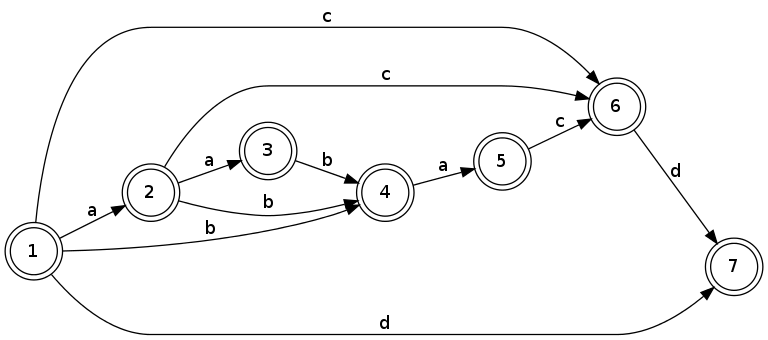
\includegraphics[width=15cm]{dawg.png}
  \caption{DAWG de "aabacd"}
  \label{fig:dawg}
\end{figure}

\bibliographystyle{plain} \bibliography{biblio}

\end{document}
